\documentclass[../doc.tex]{subfiles}

\begin{document}
\section{Instrukcja obsługi aplikacji}

\subsection{Uruchamianie}

Aby uruchomić aplikację, należy otworzyć plik z rozszerzeniem \texttt{*.html} (\texttt{index.html}) przy pomocy dowolnej przeglądarki. Po uruchomieniu interfejs użytkownika powinien wyglądać jak na rysunku \ref{fig:maze_start}.

\begin{figure}[H]
  \centering
  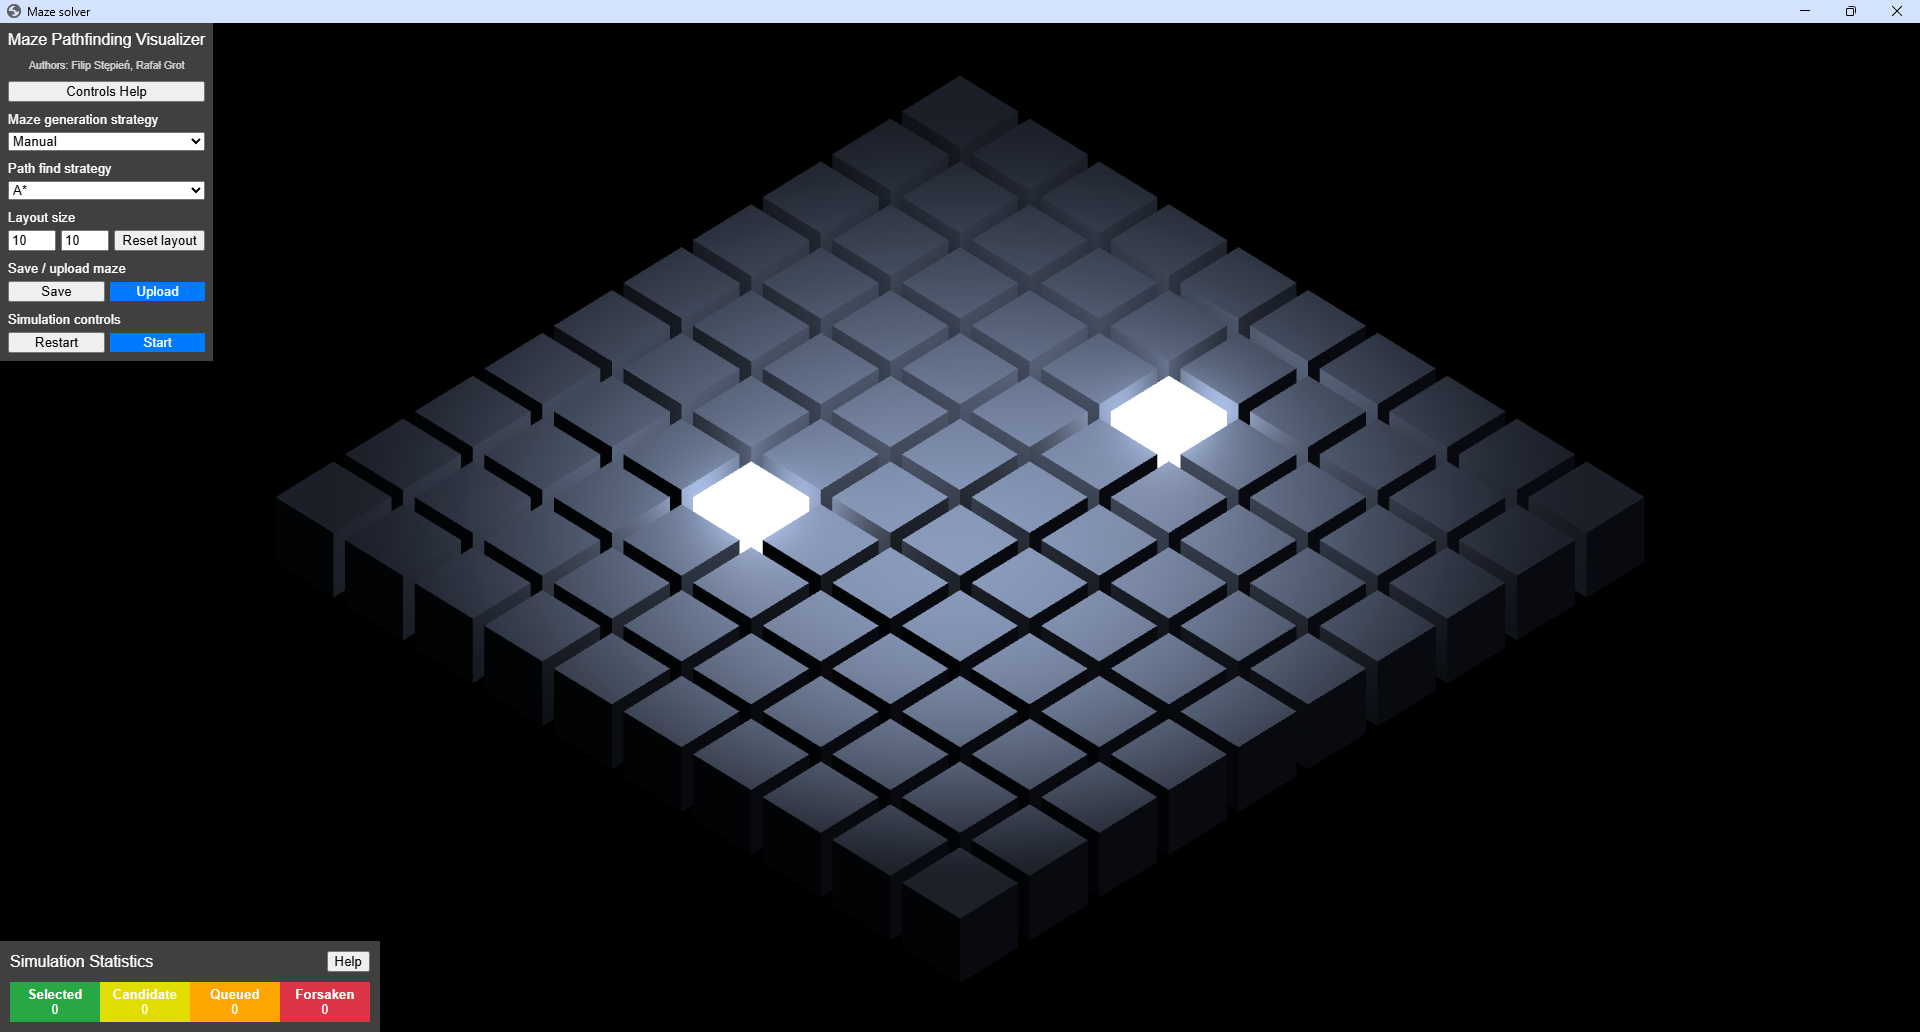
\includegraphics[width=0.85\textwidth]{figures/start.png}
  \caption{Uruchomiona aplikacja.}
  \label{fig:maze_start}
\end{figure}

\subsection{Interfejs użytkownika}

\begin{figure}[H]
  \centering
  \begin{minipage}[c]{0.35\textwidth}
    \centering
    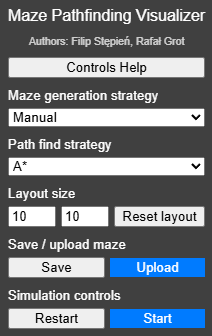
\includegraphics[width=\linewidth]{figures/controls.png}
    \caption{Panel sterowania.}
    \label{fig:control_panel}
  \end{minipage}
  \hfill
  \begin{minipage}[c]{0.6\textwidth}
    \textbf{Panel sterowania} (\cref{fig:control_panel}) zawiera wszystkie kluczowe opcje do manipulacji labiryntem:

    \begin{itemize}
      \item \textit{Controls Help} – przycisk pokazujący skróty klawiszowe.

      \item \textit{Maze generation strategy} – wybór algorytmu generowania labiryntu; opcja \textit{Manual} pozwala ręcznie stworzyć planszę.

      \item \textit{Path find strategy} – wybór algorytmu do znalezienia ścieżki.

      \item \textit{Layout size} – wybór szerokości i wysokości planszy. \textit{Reset layout} przywróci planszę do stanu początkowego.

      \item \textit{Save / upload maze} – pobieranie lub wczytywanie labiryntu z pliku.

      \item \textit{Simulation controls} – sterowanie symulacją: \textit{Restart} usuwa znaczniki wyszukanej drogi, \textit{Start} rozpoczyna wyszukiwanie drogi.
    \end{itemize}
  \end{minipage}
\end{figure}

\begin{figure}[H]
  \centering
  \begin{minipage}[c]{0.6\textwidth}
    \textbf{Plansza labiryntu} (\cref{fig:field}) stanowi główny element wizualizacji. Składa się z symetrycznych sześcianów — obecność sześcianu oznacza możliwą \textbf{drogę}, jego brak wskazuje na \textbf{ścianę}. Użytkownik może najechać kursorem na dowolne pole niebędące punktem startowym ani końcowym (oznaczone kolorem białym), co skutkuje jego podświetleniem na zielono (rysunek \ref{fig:cursor}). Kliknięcie \textbf{lewym przyciskiem myszy} usuwa drogę, natomiast \textbf{prawym} ją przywraca.

    Możliwa jest również modyfikacja położenia punktów startowego i końcowego. W tym celu należy przytrzymać klawisz \textbf{Shift} i kliknąć \textbf{prawym przyciskiem myszy}, aby zmienić pozycję startu, lub przytrzymać \textbf{Ctrl} i kliknąć \textbf{prawym przyciskiem myszy}, aby ustawić nowy punkt końcowy.

  \end{minipage}
  \hfill
  \begin{minipage}[c]{0.35\textwidth}
    \centering
    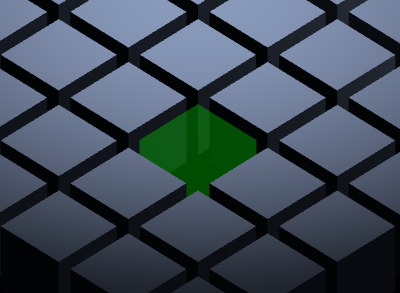
\includegraphics[width=\linewidth]{figures/cursor.png}
    \caption{\centering Wybranie oraz usunięcie pola labiryntu.}
    \label{fig:cursor}
  \end{minipage}
\end{figure}

\vspace{-9pt}

\begin{figure}[H]
  \centering
  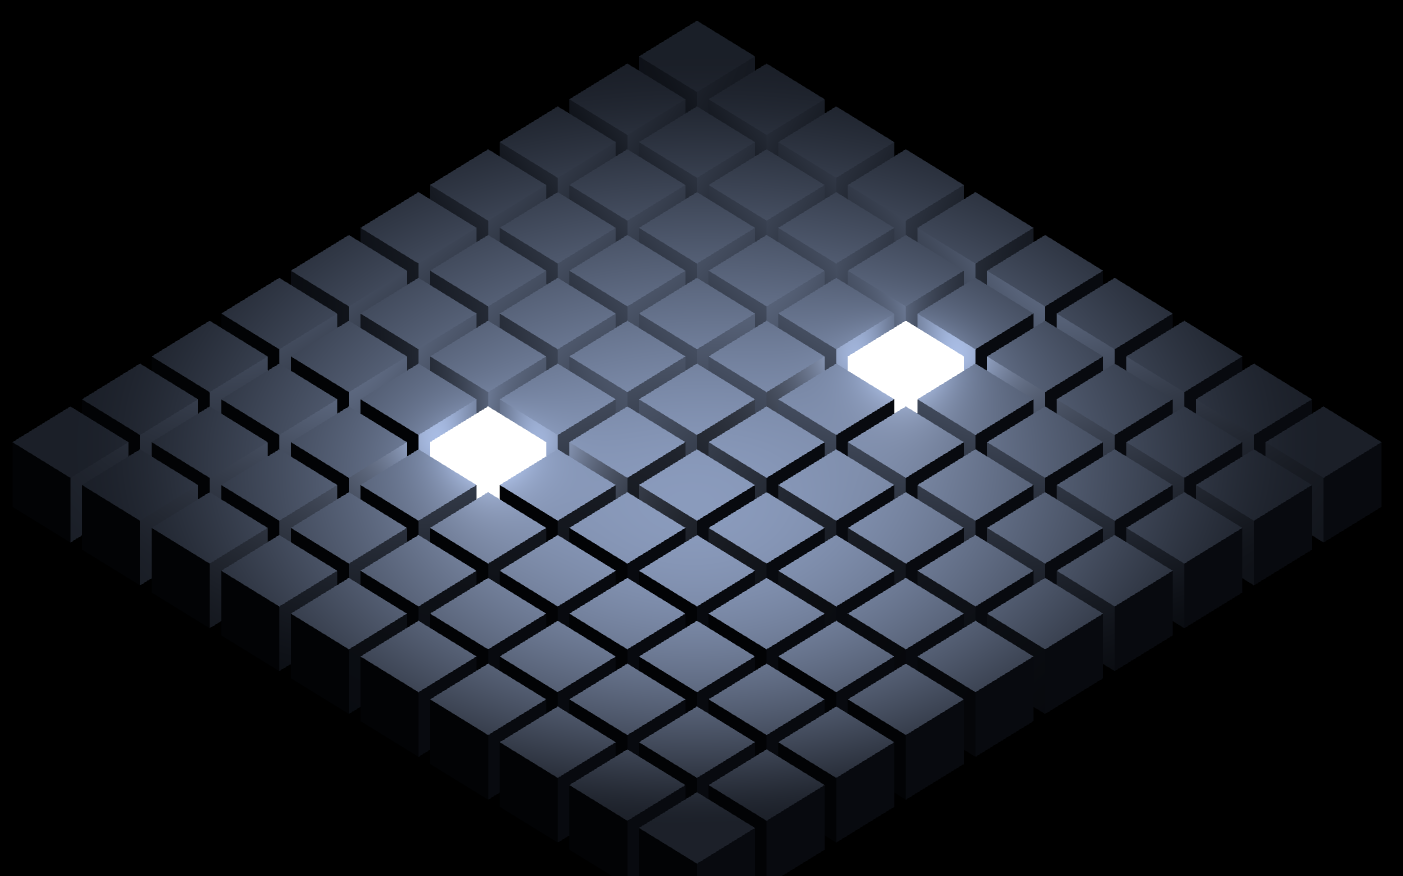
\includegraphics[width=0.85\linewidth]{figures/field.png}
  \caption{Plansza labiryntu.}
  \label{fig:field}
\end{figure}

\textbf{Panel statystyk} (\cref{fig:stats})
prezentuje liczbę pól labiryntu przypisanych do poszczególnych kategorii, (patrz: \ref{sec:node_states} \nameref{sec:node_states}), które algorytm wykorzystuje podczas poszukiwania ścieżki.



\noindent Informacja o znaczeniu poszczególnych statystyk jest zawsze dostępna po kliknięciu przycisku \textit{Help}.

\begin{figure}[H]
  \centering
  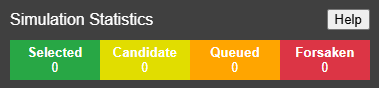
\includegraphics[width=0.6\linewidth]{figures/stats.png}
  \caption{Panel statystyk.}
  \label{fig:stats}
\end{figure}

Kolory statystyk odpowiadają barwom klasifikowanych pól w symulacji. Kolorwanie pól labiryntu podczsas pracy algorytmu przedstawiono na rysunku \ref{fig:colors}. Aktualny krok dodatkowo podświetla wybrane pole na odpowiadający mu kolor.

\begin{figure}[H]
  \centering
  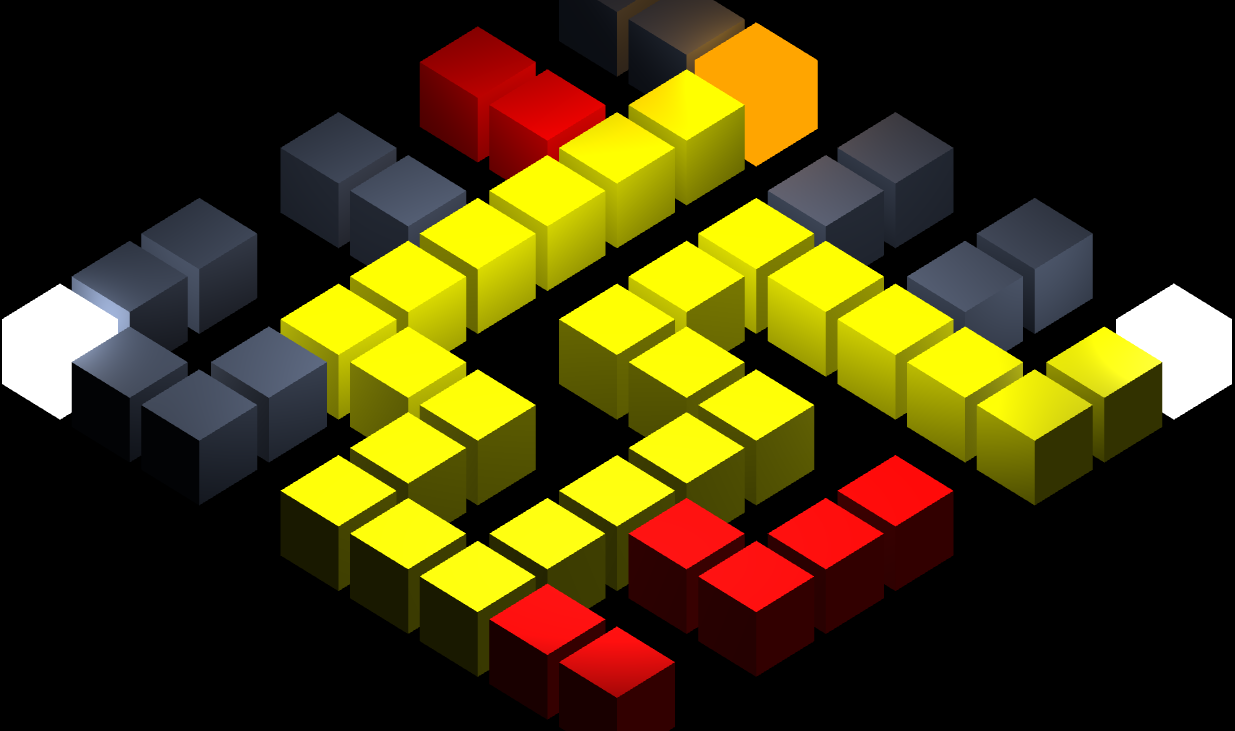
\includegraphics[width=0.85\linewidth]{figures/colors.png}
  \caption{\centering Przebieg działania algorytmu. Widoczne są pola startowe i końcowe oznaczone kolorem białym, pola \textit{Candidate} w kolorze żółtym, pola \textit{Forsaken} w kolorze czerwonym oraz pole \textit{Queued} (aktualny krok algorytmu) w kolorze pomarańczowym.}
  \label{fig:colors}
\end{figure}

\subsection{Przeprowadzanie symulacji}

Typowy przebieg czynności po uruchomieniu aplikacji wygląda następująco - wszystkie wymienione kroki wykonuje się w \textbf{panelu sterowania}:

\begin{enumerate}

  \item Wybranie algorytmu generowania labiryntu (sekcja \textit{Maze generation strategy}).

  \item Określenie wielkości planszy (sekcja \textit{Layout size}).

  \item Wylosowanie struktury planszy odpowiadającej preferencjom użytkownika (przycisk \textit{Reset layout} w sekcji \textit{Layout size}).

  \item Opcjonalne zapisanie struktury labiryntu do pliku do późniejszego wczytania (przycisk \textit{Save} w sekcji \textit{Save/upload maze}).

  \item Wybór algorytmu wyszukiwania ścieżki (sekcja \textit{Path find strategy}).

  \item Uruchomienie symulacji (przycisk \textit{Start} w sekcji \textit{Simulation controls}).

  \item Monitorowanie przebiegu algorytmu oraz analizowanie danych w \textbf{panelu statystyk}.
\end{enumerate}



\end{document}